% !TEX root =  main.tex

\clearpage

\setlength{\fboxsep}{1em}
\fbox{%
  \parbox{\textwidth}{
    \section*{\centerline{Erklärung}}

    \begin{tabbing}
      mmmmmmmmmmm     \= \kill
      \textbf{Name, Vorname:} \> Car, Christian; Kießling, Marius\\
      \textbf{Matrikelnummer:} \> \matrikelnr\\
      \textbf{Studiengang, Kurs:} \> \studiengang, \kurs\\\\
      \textbf{Titel der Arbeit:} \> \titel
      \hspace{1cm}
    \end{tabbing}

    
    Ich versichere hiermit, dass ich meine Studienarbeit mit dem Thema \textit{\titel} selbstständig verfasst und keine anderen als die angegebenen Quellen und Hilfsmittel benutzt habe.
    \linebreak\linebreak
    Falls sowohl eine gedruckte als auch elektronische Fassung abgegeben wurde, versichere ich zudem, dass die eingereichte elektronische Fassung mit der gedruckten Fassung übereinstimmt.
    
    \vspace{1cm}

    \begin{minipage}[b]{0.35\linewidth}
      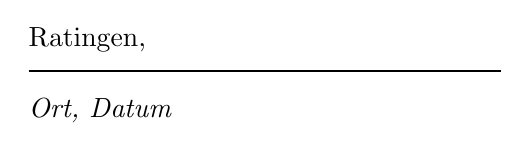
\begin{tikzpicture}[line width=0.75pt,every node/.style={inner sep=0,outer sep=0}] 
        \node[anchor=west] (field value) at (0,0.9) {Ratingen, \datumAbgabe};
        \draw[-] (0,0.5) -- (6,0.5);
        \node[anchor=west] (field title) at (0,0) {\textit{Ort, Datum}};
      \end{tikzpicture}
    \end{minipage}
    \hspace{2.5cm}
    \begin{minipage}[b]{0.35\linewidth}
      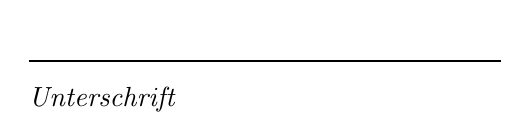
\begin{tikzpicture}[line width=0.75pt,every node/.style={inner sep=0,outer sep=0}] 
        \node[anchor=west] (field value) at (0,0.9) {};
        \draw[-] (0,0.5) -- (6,0.5);
        \node[anchor=west] (field title) at (0,0) {\textit{Unterschrift}};
      \end{tikzpicture}
    \end{minipage}
    \vspace{0.8cm}
  }
}%
